\chapter{Natural Language}

\begin{figure}[!h]
	
\includegraphics[scale=0.5]{immagini/Natural_language.png}
\end{figure}

Un \textbf{Conversational System} è un'interfaccia uomo macchina in grado di comprendere \textbf{il linguaggio umano} e condurre una conversazione scritta o verbale con l'utente. È un tipo di interfaccia usata per migliorare l'esperienza dell'utente guidandone l'interazione durante l'uso del prodotto.

La conversazione deve essere:
\begin{itemize}
	\item \textbf{Naturale}: l'utente deve poter usare un linguaggio \textbf{spontaneo}, non meccanico o verboso.
	\item \textbf{Accessibile}: l'utente deve capire facilmente e senza nessuna fatica come interagire con l'interfaccia.
	\item \textbf{Efficiente}.
\end{itemize}

Il primo problema che un programmatore deve affrontare quando vuole implementare un'interfaccia del genere è  il seguente: il \textbf{linguaggio naturale è ambiguo}, infatti si possono usare molti costrutti per esprimere il medesimo concetto o impartire il medesimo comando.

Un servizio efficiente per poter scavalcare questo problema è \textbf{Amazon Lex}.

Amazon Lex si basa su due concetti fondamentali: \textbf{speech recognition} e \textbf{natural language understanding}.
Benché esistano molti modi per esprimere il medesimo concetto, un servizio di riconoscimento vocale \textbf{deve essere in grado di capire} ciò che vogliamo fare e quale sia il nostro obiettivo.

Si indicherà con il termine \textbf{intento} l'obbiettivo dell'utente.
Per poter soddisfare l'intento, si deve fare in modo che il sistema riconosca delle \textbf{informazioni chiave} per comprendere il comando. Queste informazioni chiave prendono il nome di \textbf{slots}.

Gli \textbf{slots} sono quindi i dati necessari al conversational system per soddisfare la richiesta dell'utente.

Inoltre per aiutare il sistema ad interagire con gli utenti e a riconoscere il comando si definiscono anche delle \textbf{utterances}, ovvero delle frasi di esempio con diversa struttura ma uguale significato. Un insieme di \textbf{utterances} fa riferimento ad un \textbf{intento}.

Infine si procede a definire la sequenza d'interazione tra l'utente e il conversational system  fornendo a quest ultimo dei \textbf{prompts}, ovvero la risposta che l'interfaccia darà all'utente dopo ogni comando ricevuto.

\pagebreak

\textbf{AWS Lambda} è una piattaforma di calcolo \textbf{event-driven} e \textbf{serverless} che Amazon fornisce come parte dei suoi \textbf{servizi web}: mette in esecuzione del codice in risposta ad eventi e ne gestisce le risorse computazionali.

\begin{figure}[!h]
	\centering
	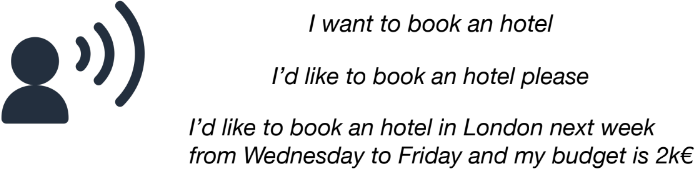
\includegraphics[scale=0.55]{immagini/Lex_general3.png}
	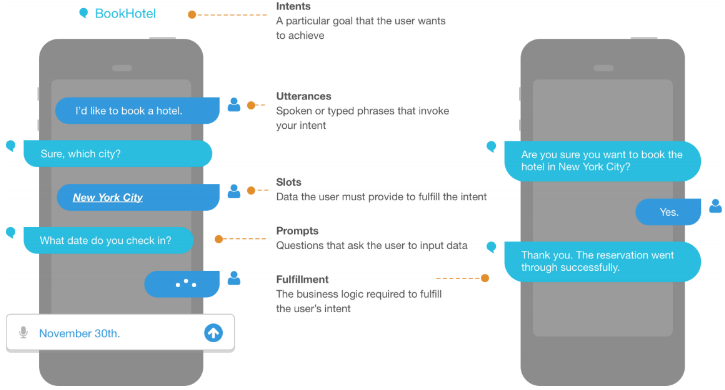
\includegraphics[scale=0.65]{immagini/Lex_general.png}
	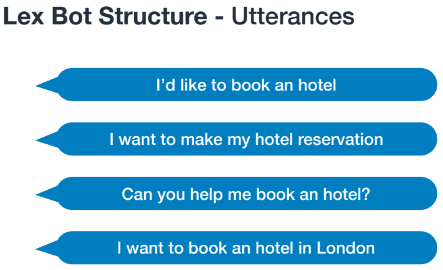
\includegraphics[scale=0.6]{immagini/Lex_general1.png}
	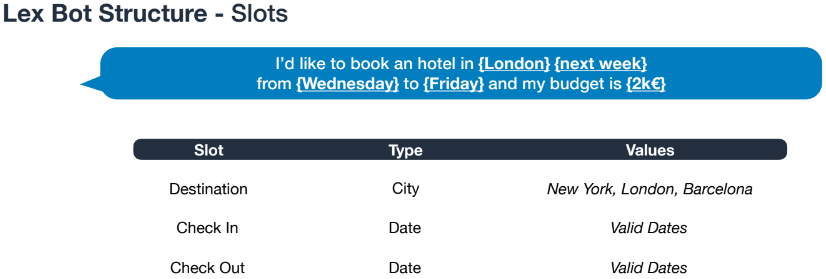
\includegraphics[scale=0.5]{immagini/Lex_general2.png}
\end{figure}
